\documentclass[a4paper,10pt,openright,openbib]{article}
\usepackage[portuges]{babel}
\usepackage[T1]{fontenc}
\usepackage{ae}
\usepackage[utf8]{inputenc}
\usepackage[pdftex]{graphicx}
\usepackage{url}
\usepackage{listings}
\usepackage{verbatim}
\usepackage{enumerate}
\usepackage[pdftex, bookmarks, colorlinks, linkcolor=black, urlcolor=blue]{hyperref} 
\usepackage[a4paper,left=2.5cm,right=2.5cm,top=3.5cm,bottom=3.5cm]{geometry}
\usepackage{colortbl}
\usepackage[margin=10pt,font=small,labelfont=bf]{caption}
\usepackage{mdwlist}
\usepackage{cleveref}
\usepackage{epsfig}



\setlength{\parindent}{0cm}
\setlength{\parskip}{2pt}


\begin{document}

%% Roofline%%
\section{Roofline}
\subsection{Machines Profile}
The machines used for this study were a MacBook Pro late 2008 and a HP dv6-2190ep from 2010.
The information about the machines were gathered from \emph{/proc/cpuinfo}, \emph{/proc/meminfo}, the \emph{Intel Ark} and \emph{Crucial} websites, with \emph{dmidecode} and \emph{sysctl} linux tools and with \emph{bandwidth} package.

\subsubsection{Peaks}
In order to calculate the rooflines, we needed the Floating-Point(FP) Performance Peak and the Memory Bandwidth's Peak. 
To attain the FP Performance Peak we calculate the following formula:

$$\mathrm{GFlop/s_{max}} =  \#_{\mathrm{cores}} \times f_{\mathrm{clock}} \times \#_{\mathrm{SIMD}}$$

MacBook Pro FP Performance Peak:
$$\mathrm{GFlop/s_{max}} =  2 \times 2.8 \times 8
						 =  44.8 GFLOPS\\s$$
HP Pavillion FP Performance Peak:
$$\mathrm{GFlop/s_{max}} =  4 \times 1.6 \times 8
						 =  51.2 GFLOPS\\s$$
\\
\\
To calculate de Memory Bandwidth Peak we resolve the following formula:

$$\mathrm{BW_{max}} =  \#_{\mathrm{channels}} \times mem_{\mathrm{clock}} \times bus_{\mathrm{bandwidth}}$$
 
MacBook Pro Memory Bandwidth Peak:
$$\mathrm{GFlop/s_{max}} =  2 \times 1067 \times 64
						 =  17.072 GB\\byte$$
HP Pavillion Memory Bandwidth Peak:
$$\mathrm{GFlop/s_{max}} =  2 \times 1333 \times 64
						 =  21.328 GB\\byte$$

\subsubsection{Specifications}
The specifications of the MacBook Pro are displayed on \autoref{tab:mbp}. \\

\begin{table}[!htp]
		\begin{tabular}{lrl}
			\hline 
			\textbf{Manufacter:} & Apple \\
			\hline \\
			\textbf{Model:} & MacBook Pro late 2008 \\
			\hline 
			\textbf{Processor} & & \\
			Manufacturer: & Intel & \\
			Arch: & Core & \\
			Model: & Core 2 Duo T9600 & \\
			Cores: & 2 & \\
			Clock Frequency: & 2.80 GHz & \\
			FP Performance's Peak: & 44.8 GFlops/s & \\
			\hline 
			\textbf{Cache} & & \\
			Level: & 1 & \\
			Size: & 32KB + 32KB & \\
			Line Size: & 64 B & \\
			Associative: & 8-way & \\
			Memory Access Bandwidth: & 40 GB/s & \\
			\\
			Level: & 2 & \\
			Size: & 6 MB & \\
			Line Size: & 64 B & \\
			Associative: & 24-way & \\
			\hline 
			\textbf{RAM} \\
			Type: & SDRAM DDR3 PC3-8500 & \\
			Frequency: & 1067 MHz & \\
			Size: & 4 GB & \\
			Num. Channels: & 2 & \\
			Latency: & 13.13 ns & \\
		\end{tabular}
		\caption{MacBook Pro late 2008 specifications}
		\label{tab:mbp}
\end{table}
The specifications of the HP dv6-2190ep are displayed on \autoref{tab:hp}. \\
\begin{table}[!htp]
		\begin{tabular}{lrl}
			\hline 
			\textbf{Manufacter:} & HP \\
			\hline 
			\textbf{Model:} & Pavillion dv6-2190ep \\
			\hline 
			\textbf{Processor} & & \\
			Manufacturer: & Intel & \\
			Arch: & Nehalem & \\
			Model: & i7-720QM & \\
			Cores: & 4 & \\
			Clock Frequency: & 1.60 GHz & \\
			FP Performance's Peak: & 51.2 GFlops/s & \\
			\hline 
			\textbf{Cache} & & \\
			Level: & 1 & \\
			Size: & 32KB + 32KB & \\
			Line Size: & 64 B & \\
			Associative: & 4/8-way & \\
			Memory Access Bandwidth: & 22 GB/s & \\
			\\
			Level: & 2 & \\
			Size: & 256 KB & \\
			Line Size: & 64 B & \\
			Associative: & 8-way & \\
			\\
			Level: & 3 & \\
			Size: & 6 MB & \\
			Line Size: & 64 B & \\
			Associative: & 12-way & \\
			\hline 
			\textbf{RAM} \\
			Type: & SDRAM DDR3 PC3-10600 & \\
			Frequency: & 1333 MHz & \\
			Size: & 4GB & \\
			Num. Channels: & 2 & \\
			Latency: & 13.5 ns & \\
		\end{tabular}
		\caption{HP Pavillion dv6-2190ep specifications}
		\label{tab:hp}
\end{table}


\subsection{Roofline Model}
\subsubsection{MacBook Pro Roofline}
\begin{figure}[!htp]
	\centering
	\begin{minipage}[t]{0.5\linewidth}
		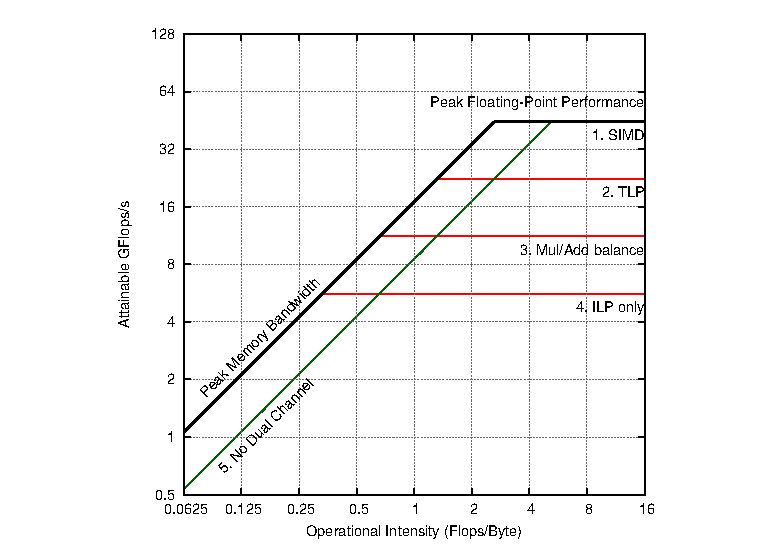
\includegraphics[width=\textwidth]{images/roofline_mbp.eps}
		\caption{Mackbook Pro late 2008 \label{fig:roofline1}}
	\end{minipage}
\end{figure}
\subsubsection{HP Pavillion Roofline}
\begin{figure}[!htp]
	\centering
	\begin{minipage}[t]{0.5\linewidth}
		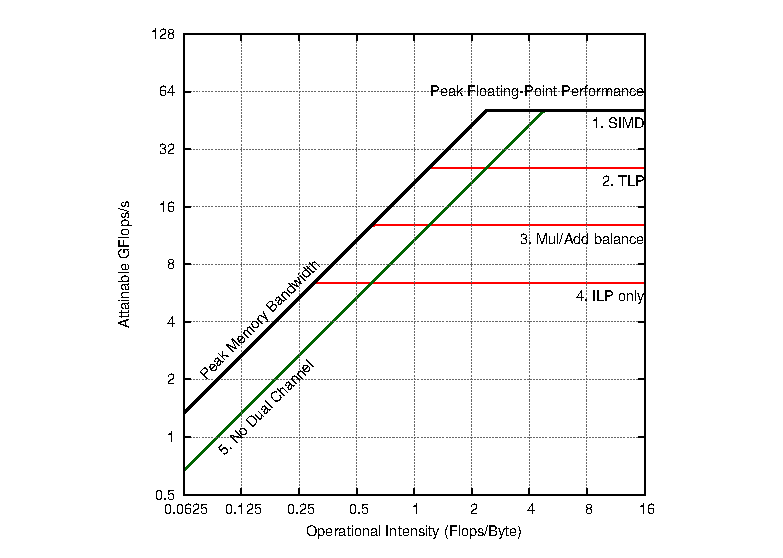
\includegraphics[width=\textwidth]{images/roofline_hp.eps}
		\caption{HP Pavillion dv6-2190ep Roofline \label{fig:roofline2}}
	\end{minipage}
\end{figure}

\subsubsection{Ceilings}
As suggested by the Roofline paper we added several ceilings to understand wich optimizations we may perform.
This ceilings were given by recalculating the roofline without some key charateristics.
\begin{description}
\item[Peak floating-point performance] The roofline, where all components and features are considered.
\item[]
\item[]
\item[]
\end{description}
For memory only one ceiling was calculated, besides the roofline.
\begin{description}
\item[Peak stream bandwidth] The roofline, where all features are considered.
\item[One-channel]
\end{description}

\section{PAPI Case Study}
\subsection{Problem}
The case study of this report, is to analyse the performance of a \textbf{matrix multiplication} algorithm, \begin{equation}Matrix A * Matrix B = Matrix C\end{equation} wich contains a triple nested loop with the indexes i,j and k(line,column and position). Our implementation will explore the index order \textbf{i,j,k} of the triple nested loop.

\subsection{Algorithm Analysis}
The implementation produced to calculate the matrix multiplication was made in C and compiled with Optimization level 1 (-o).
The algorithm of matrix multiplication is presented here, in order to better understand the problem at hand.

\begin{verbatim}
for (i = 0; i < size; i++) {
    for (j = 0; j < size; j++) {
        for(k = 0; k < size; k++) {
            acc += matrixA[i][k] * matrixB[k][j];				
            }		
            matrixC[i][j] = acc;	
            acc = 0;
        }
    }
\end{verbatim}

Two versions of the program were run, one with the matrixB and other with the transpose matrixB. With this second version, it is expected that the positions used in the algorithm will be contiguous, reducing the number of accesses to memory. 

\subsection{Counters Used}
To measure the algorithm's perfomance, hardware counters were used. To gather the information of these counters we used \emph{PAPI}(Performance API). This tool alowed us to measure the following counters:
\begin{description}
\item[PAPI \_TOT\_CYC] Total number of cycles;
\item[PAPI \_TOT\_INS] Instructions completed;
\item[PAPI \_LD\_INS] number of load instructions;
\item[PAPI \_SR\_INS] number of store instructions;
\item[PAPI \_FP\_OPS] Floating point operations;
\item[PAPI \_FP\_INS] Floating point instructions;
\item[PAPI \_L1\_DCA] L1 data cache accesses;
\item[PAPI \_L1\_DCM] L1 data cache misses;
\item[PAPI \_L2\_DCA] L2 data cache accesses;
\item[PAPI \_L2\_DCM] L2 data cache misses;
\item[PAPI \_L3\_DCA] L3 data cache accesses;
\end{description}

\subsection{Tests}
The four tests, presented below, were chosen to run in the two different version(normal and transpose). Each test was run four times, with the best execution time being select as long as the range was no larger than the other three. Each test fits in a different memory level(L1, L2, L3 and RAM).   
\begin{table}[!htp]
	\center{
	\begin{tabular}{lrlrlrl}
		\hline
		\textbf{Memory} & \textbf{Size} & \textbf{Matrix Size} \\
		\hline
		L1 & 30 KB & 50 \\
		L2 & 255 KB & 146 \\
		L3 & 3 MB & 500 \\
		RAM & 7.68 MB & 800 \\
		\hline
	\end{tabular}
	\caption{Test cases}
	\label{tab:testcases}
	}
\end{table}
\subsection{Results}
\subsubsection{Analysis Chache}

 To measure the data cache misses the counters PAPI\_L1\_DCM and PAPI\_L2\_DCM were used.

\begin{figure}[!htp]
	\centering
	\begin{minipage}[t]{0.5\linewidth}
		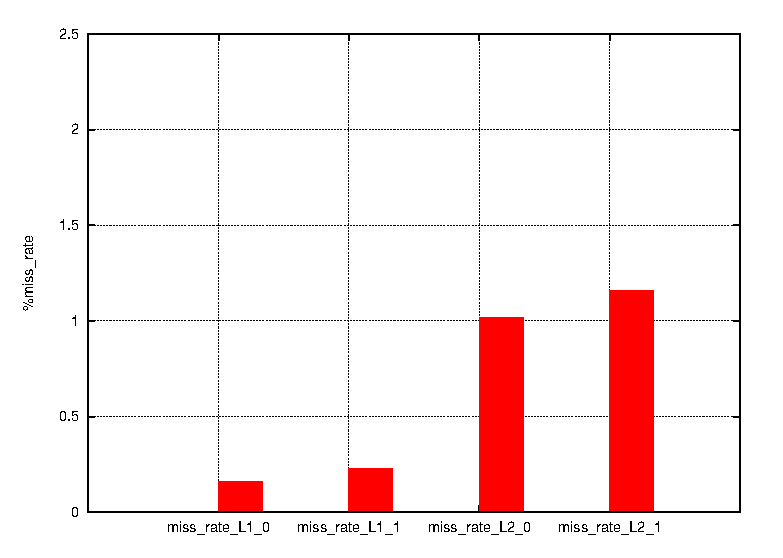
\includegraphics[width=\textwidth]{images/caches.eps}
		\caption{Percentage of Cache Misses \label{fig:cachel1}}
	\end{minipage}
\end{figure}

The above graphic shows an increase of percentage of misses with the optimized version, they are misleading. The next graph shows that although the percentage of misses increased, the total of misses didn't because the number of accesses also droped.

\begin{figure}[!htp]
	\centering
	\begin{minipage}[t]{0.5\linewidth}
		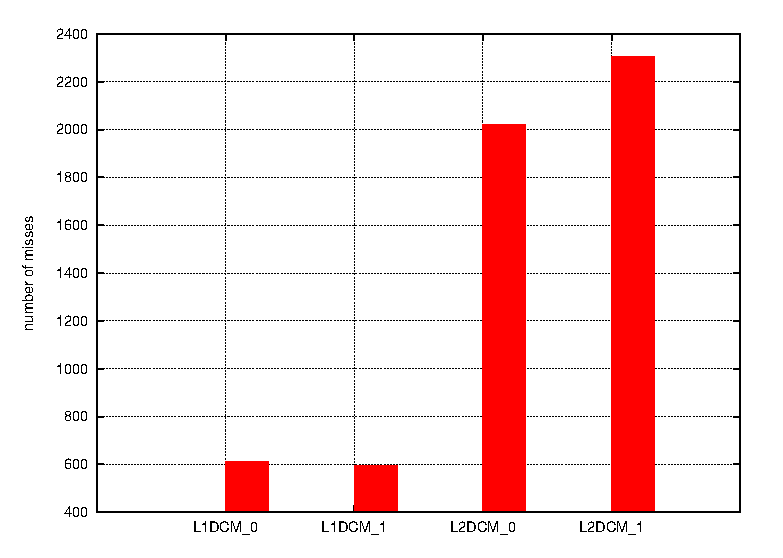
\includegraphics[width=\textwidth]{images/misses.eps}
		\caption{Number of Cache Misses \label{fig:cachel1}}
	\end{minipage}
\end{figure} 

Usage of both levels of cache was estimated with specific counters. PAPI\_L1\_DCA and PAPI\_L2\_DCA provided the number of data accesses to the caches.

Before the results were out, it was expected a decrease of cache accesses from version one to version two of the algorithm.

\begin{figure}[!htp]
	\centering
	\begin{minipage}[t]{0.5\linewidth}
		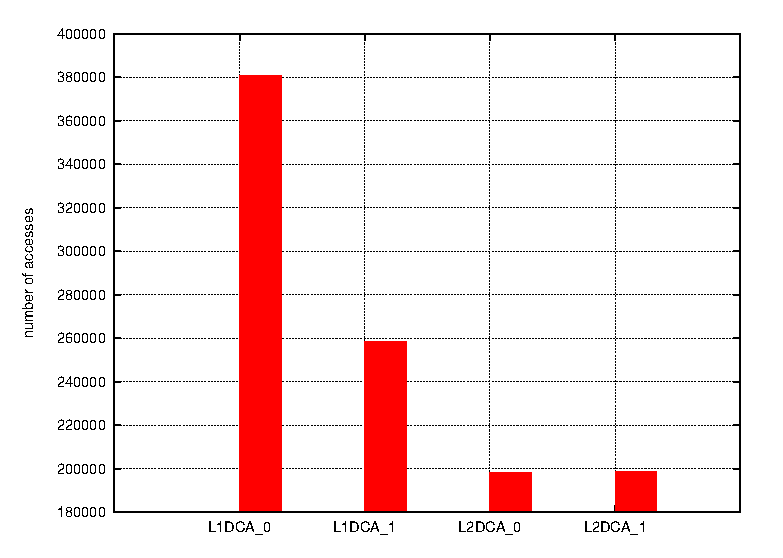
\includegraphics[width=\textwidth]{images/totals.eps}
		\caption{Number of Memory Accesses \label{fig:cachel1}}
	\end{minipage}
\end{figure}

As we can see, the number of access to cache drops significantly from the first version to the second version while running with the L1 Cache Test. Though in the second test, the L2 Cache, the number of accesses slightly increased.


\begin{thebibliography}{9}
\bibitem{roofline}
	\texttt{\small
	Roofline: An insightful Visual Performance Model for Floating-Point Programs and Multicore Architectures}	\\
	\emph{Samuel Webb Williams, Andre Waterman, David A. Patterson}	\\
	23th November 2012

\bibitem{ark}
	\texttt{\small
	http://ark.intel.com/products/35563/Intel-Core2-Duo-Processor-T9600-6M-Cache-2\_80-GHz-1066-MHz-FSB}	\\
	\emph{Intel{\textregistered} Core {\texttrademark} 2 Duo Processor T9600 (6M Cache, 2.80 GHz, 1066 MHz FSB)}	\\
	{\copyright}Intel Corporation	\\
	23th November 2012

\bibitem{ark2}
	\texttt{\small
	http://ark.intel.com/products/43122/Intel-Core-i7-720QM-Processor-6M-Cache-1\_60-GHz}	\\
	\emph{Intel{\textregistered} Core {\texttrademark} i7-720QM Processor(6M Cache, 1.60 GHz)}	\\
	{\copyright}Intel Corporation	\\
	23th November 2012

\bibitem{crucial}
	\texttt{\small
	http://www.crucial.com/store/ListParts.aspx?model=MacBook\%20Pro\%20\%28Early\%202008\%20and\%20Late\%202008\%29}	\\
	\emph{Computer memory upgrades for Apple MacBook Pro (Early 2008 and Late 2008) Laptop/Notebook from Crucial.com }	\\
	{\copyright} Micron Technology	\\
	24th November 2012

\bibitem{crucial2}
	\texttt{\small
	http://www.crucial.com/store/listparts.aspx?model=Pavilion\%20dv6-2190ep\&Cat=RAM}	\\
	\emph{Computer memory upgrades for HP - Compaq Pavilion dv6-2190ep Laptop/Notebook from Crucial.com}	\\
	{\copyright} Micron Technology	\\
	24th November 2012	

\end{thebibliography}

\end{document}


